%%%%%%%%%%%%%%%%%%%%%%%%%%%%%%%%%%%%%%%%%
% "ModernCV" CV and Cover Letter
% LaTeX Template
% Version 1.11 (19/6/14)
%%%%%%%%%%%%%%%%%%%%%%%%%%%%%%%%%%%%%%%%%

\documentclass[11pt,a4paper,sans]{moderncv}

\usepackage[utf8]{inputenc}
\usepackage[export]{adjustbox}
\usepackage{multicol}

\moderncvstyle{casual} % CV theme - options include: 'casual' (default), 'classic', 'oldstyle' and 'banking'
\moderncvcolor{blue} % CV color - options include: 'blue' (default), 'orange', 'green', 'red', 'purple', 'grey' and 'black'

\usepackage{color}
\usepackage{lipsum}
\usepackage[scale=0.90]{geometry}

\setlength{\hintscolumnwidth}{4cm}

\firstname{Shelley}
\familyname{Vohr}

\title{Curriculum Vitae}

% This command effectively comments out anything within it
\newcommand{\comment}[1]{} 

%----------------------------------------------------------------------------------------

\begin{document}

\textit{\Huge{\textcolor{black}{Shelley Vohr}}}

\hrulefill

%--------------------------------------
%	CONTACT
%--------------------------------------

\begin{multicols}{2}
  \section{Contact}
  \cvitem{Mobile}{+1 (843) 670-5793}
  \cvitem{Email}{codebytere@gmail.com}
  \cvitem{Website}{http://codebyte.re}
  \cvitem{GitHub}{https://github.com/codebytere}
  \columnbreak
  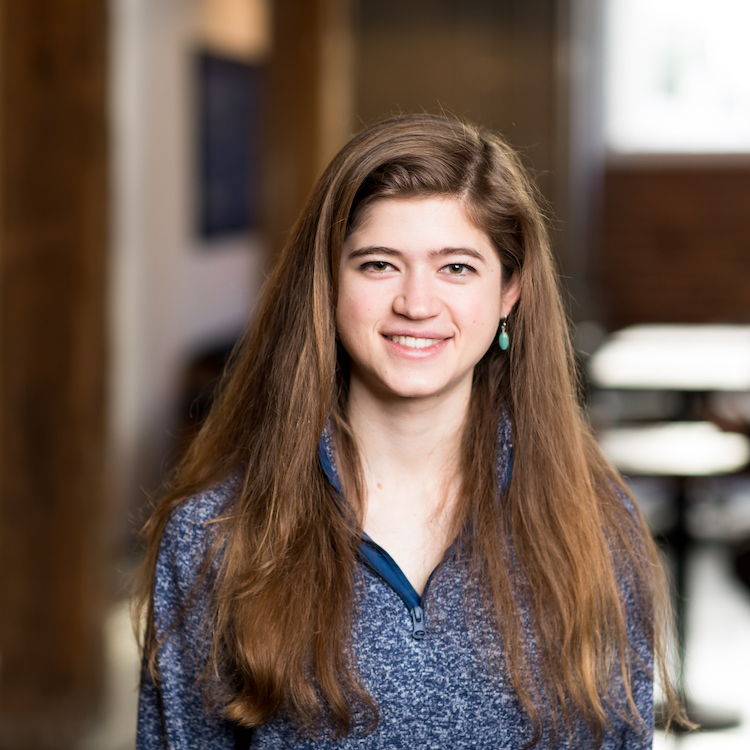
\includegraphics[width=27mm, right]{headshot.jpg}
\end{multicols}

%---------------------------------------
%	WORK EXPERIENCE
%---------------------------------------

\section{Work Experience}

\cvitem{Feb. 2019 -- Present}{\textbf{GitHub} \textit{San Francisco, CA} -- Software Engineer 3}
\renewcommand{\listitemsymbol}{\textcolor{black}{-~}}
\cvlistitem{Improved, and maintained Electron for the over 100M desktops that rely on Electron as part of their favorite suite of applications}
\cvlistitem{Ensured that Electron releases were published on time and built automation tooling as the Chair of the Releases Working Group}
\cvlistitem{Led development on suite of bots to handle everything from backporting to automated deploys using 2 Factor Authentication via chatops}
\cvlistitem{Top contributor to the core Electron repository since August 2017 with over 650 substantive merged and shipped pull requests}
\cvlistitem{Streamlined and released new versions of Node.js as a member of the Node.js LTS Release Team and Node.js Core Collaborator}

\cvitem{Sep. 2017 -- Feb. 2019}{\textbf{GitHub} \textit{San Francisco, CA} -- Software Engineer 2}
\renewcommand{\listitemsymbol}{\textcolor{black}{-~}}
\cvlistitem{Worked as a member of the Electron.js core team to add features and review feature requests, pull requests, and triage issues reported by the community.}

\cvitem{May 2017 -- Aug. 2017}{\textbf{GitHub} \textit{San Francisco, CA} -- Software Engineering Intern}
\renewcommand{\listitemsymbol}{\textcolor{black}{-~}}
\cvlistitem{Improved performance and repository visibility permissions on GitHub and GitHub Enterprise.}
\cvlistitem{Built an API to surface repository dependency data for users on GitHub and GitHub Enterprise.}

\cvitem{May 2016 -- Aug. 2016}{\textbf{IFTTT} \textit{San Francisco, CA} -- Software Engineering Intern}
\renewcommand{\listitemsymbol}{\textcolor{black}{-~}}
\cvlistitem{Worked with Javascript and Ruby on Rails alongside members of the web team as they developed and launched several new products within the IFTTT ecosystem.}

\cvitem{Sep. 2015 -- Dec. 2015}{\textbf{Transloc} \textit{Durham, NC} -- Software Engineering Intern}
\renewcommand{\listitemsymbol}{\textcolor{black}{-~}}
\cvlistitem{Worked with Javascript and Python to develop portions of the Traveler transit analysis product and built web tools for internal use within the company.}

\cvitem{May 2015 -- Aug. 2015}{\textbf{Embedly (acq. by Medium)} \textit{Boston, MA} -- Software Engineering Intern}
\renewcommand{\listitemsymbol}{\textcolor{black}{-~}}
\cvlistitem{Used front-end development tools including Ember.js and Python to create a fully-featured administrative backend and significant portions of a new version of the company's web app.}

\comment {
  \cvitem{Jan. 2017 -- May 2017}{\textbf{Duke University} \textit{Durham, NC} -- Undergraduate Teaching Assistant}
  \renewcommand{\listitemsymbol}{\textcolor{black}{-~}}
  \cvlistitem{Assisted students in learning concepts of discrete math as they relate to computer science as well as grading assessments and coding assignments.}
}

%---------------------------------------
%	EDUCATION
%---------------------------------------

\section{Education}

\cvitem{Aug 2014 -- May 2018}{\textbf{Duke University} \textit{Durham, NC} \newline { Bachelor in Computer Science \textit{GPA - 3.55/4.00}}}

%------------------------------------
%	SKILLS
%------------------------------------

\section{Skills}

\cvitem{\textbf{Experienced}}{C++, JavaScript, Objective-C, HTML5/CSS3}
\cvitem{\textbf{Intermediate}}{Ruby on Rails, Python, Git, Bash, TypeScript, C}

%------------------------------------
%	SPEAKING MERITS
%------------------------------------

\comment {
  \section{Speaking Merits}

  \cvitem{}{JSHeroes -- Apr. 2019}
  \cvitem{}{Modern JS /Runtimes/ -- Mar. 2019}
  \cvitem{}{Node Collaborator Summit -- Nov. 2018}
  \cvitem{}{JSConfEU - Jun. 2018}
  \cvitem{}{Node Summit -- Jun. 2018}
  \cvitem{}{Nodevember -- Nov. 2017}
  \cvitem{}{GitHub Universe -- Oct. 2017}
}

\end{document}